% !TEX program = xelatex
% !TEX encoding = UTF-8 Unicode
%
% SPDX-License-Identifier: CC-BY-4.0
% Group: 2026-Fan-Lee-Liu
% Merged Version v3: Layout Fix for System Architecture

\documentclass[aspectratio=169]{beamer}

% --- THEME SETUP ---
\mode<presentation>{
    \usetheme{NordlingLab169}
}

% --- PACKAGES ---
\usepackage[english]{babel}
\usepackage{graphicx}
\usepackage{booktabs}
\usepackage{tikz}
\usetikzlibrary{shapes.geometric, arrows, positioning}

% --- TIKZ SETTINGS (FIXED: Added text width to force wrapping) ---
\tikzset{
    agent/.style={rectangle, rounded corners, minimum width=2.5cm, minimum height=1.2cm, text centered, text width=2.2cm, draw=black, fill=blue!10},
    arrow/.style={thick,->,>=stealth, line width=1.5pt}
}

% --- FONT SETTINGS ---
\usepackage{helvet}
\renewcommand{\familydefault}{\sfdefault}

% --- METADATA ---
\title[Agentic ECG Detection]{Agentic ECG-Based Fatigue and Stress Detection}
\subtitle{Agentic AI Course - Final Presentation}
\author[Fan, Lee, Liu]{Fan,~Cheng-Yu \and Lee,~Po-Lin \and Liu,~Wu-Jun}
\institute[NCKU]{
    National Cheng Kung University\\
    Agentic AI Course
}
\date{Spring 2026}

\begin{document}

% =======================================================
% SLIDE 1: TITLE PAGE
% =======================================================
\setbeamertemplate{background}[NLTitle]
\setbeamertemplate{footline}[NLTitle]
\begin{frame}
    \titlepage
\end{frame}

% =======================================================
% OUTLINE SETUP
% =======================================================
\section{Problem \& Motivation}
\section{System Architecture}
\section{Demo \& Results}
\section{Challenges \& Lessons Learned}
\section{Conclusion}

% =======================================================
% SLIDE 2: OUTLINE
% =======================================================
\setbeamertemplate{background}[NLCC]
\setbeamertemplate{footline}[NLCC]
\begin{frame}{Outline}
    \tableofcontents
\end{frame}

% =======================================================
% SECTION 1: PROBLEM & MOTIVATION
% =======================================================
\begin{frame}{Problem Statement}
    \begin{itemize}
        \item \textbf{Data Complexity:} ECG signals contain physiological info related to fatigue/stress, but raw data is hard to interpret directly.
        \item \textbf{Need for Automation:} Manual analysis is slow; an automated and interpretable decision mechanism is required.
        \item \textbf{Gap:} Current systems lack "Agentic" capabilities to provide actionable feedback.
    \end{itemize}
\end{frame}

\begin{frame}{Motivation}
    Why choose this approach?
    \vspace{1em}
    \begin{itemize}
        \item \textbf{Time-Domain HRV:} Features like RMSSD are computationally simple yet clinically explainable.
        \item \textbf{Efficiency:} CSV-based ECG data allows for rapid processing pipelines.
        \item \textbf{Agentic AI:} Moves beyond simple detection to enable decision-making and actionable feedback (e.g., "Take a break").
    \end{itemize}
\end{frame}

% =======================================================
% SECTION 2: ARCHITECTURE (FIXED LAYOUT)
% =======================================================
\begin{frame}{System Architecture: The Agentic Workflow}
    The system follows a \textbf{Perception $\rightarrow$ Reasoning $\rightarrow$ Action} loop:

    \vspace{0.5em}
    \centering
    % 使用 resizebox 強制將圖表寬度限制在 90% 的頁面寬度內
    \resizebox{0.9\textwidth}{!}{%
    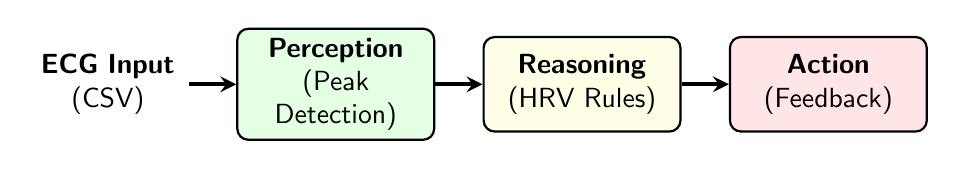
\begin{tikzpicture}[node distance=0.6cm, auto, thick] 
        
        % Nodes
        \node (input) [text width=1.8cm, align=center] {\textbf{ECG Input}\\(CSV)};
        
        \node (perception) [agent, right=of input, fill=green!10] {\textbf{Perception}\\(Peak Detection)};
        
        \node (reasoning) [agent, right=of perception, fill=yellow!10] {\textbf{Reasoning}\\(HRV Rules)};
        
        \node (action) [agent, right=of reasoning, fill=red!10] {\textbf{Action}\\(Feedback)};
        
        % Arrows
        \draw[arrow] (input) -- (perception);
        \draw[arrow] (perception) -- (reasoning);
        \draw[arrow] (reasoning) -- (action);
        
    \end{tikzpicture}
    }
    
    \vspace{1em}
    \raggedright % 恢復靠左對齊
    \footnotesize
    \begin{itemize}
        \item \textbf{Perception:} Signal loading, cleaning, and R-Peak detection.
        \item \textbf{Reasoning:} Calculating BPM/RMSSD and evaluating physiological state.
        \item \textbf{Action:} Generating human-readable recommendations (e.g., Warning).
    \end{itemize}
\end{frame}

% =======================================================
% SECTION 3: DEMO & RESULTS
% =======================================================
\begin{frame}{Methodology: Time-Domain Metrics}
    We utilize Time-Domain features for robust detection:
    \vspace{1em}
    \begin{table}
        \centering
        \begin{tabular}{ll}
            \toprule
            \textbf{Metric} & \textbf{Description} \\
            \midrule
            \textbf{BPM} & Mean heart rate derived from RR intervals. \\
            \textbf{SDNN} & Overall heart rate variability (Standard Deviation). \\
            \textbf{RMSSD} & Root Mean Square of Successive Differences (Short-term). \\
            \bottomrule
        \end{tabular}
    \end{table}
\end{frame}

\begin{frame}{Advanced Methodology: Frequency-Domain}
    In addition to Time-Domain, we analyze spectral density for deeper insights:
    \vspace{1em}
    \begin{table}
        \centering
        \begin{tabular}{lcl}
            \toprule
            \textbf{Feature} & \textbf{Frequency (Hz)} & \textbf{Physiological Meaning} \\
            \midrule
            \textbf{LF} & 0.04 -- 0.15 & Sympathetic / Stress \\
            \textbf{HF} & 0.15 -- 0.40 & Parasympathetic / Relax \\
            \textbf{LF/HF} & - & Autonomic Balance \\
            \bottomrule
        \end{tabular}
    \end{table}
    
    \vspace{0.5em}
    \small
    \textit{Note: A high LF/HF ratio typically indicates sympathetic dominance (Stress).}
\end{frame}

\begin{frame}{Agent Decision Logic}
    The Reasoning Agent applies the following threshold rules:
    \vspace{1em}
    
    \begin{columns}
        \column{0.33\textwidth}
        \begin{block}{High Stress}
            \centering
            \textbf{BPM $>$ 100}\\
            AND\\
            \textbf{RMSSD $>$ 100}
        \end{block}
        
        \column{0.33\textwidth}
        \begin{block}{Fatigue}
            \centering
            \vspace{0.8em}
            \textbf{RMSSD $<$ 30}\\
            (Low Variability)
            \vspace{0.8em}
        \end{block}
        
        \column{0.33\textwidth}
        \begin{block}{Normal State}
            \centering
            \vspace{0.8em}
            \textbf{Otherwise}\\
            (Baseline)
            \vspace{0.8em}
        \end{block}
    \end{columns}
\end{frame}

% =======================================================
% SECTION 4: CHALLENGES & LESSONS
% =======================================================
\begin{frame}{Challenges}
    \begin{itemize}
        \item \textbf{Signal Quality:} Simplified R-peak detection is sensitive to noise; lacks clinical annotations for verification.
        \item \textbf{Data Assumptions:} Currently assumes a fixed sampling rate, which varies in real-world devices.
        \item \textbf{Generalization:} Threshold-based rules (e.g., RMSSD < 30) lack personalization for different users (athletes vs. non-athletes).
    \end{itemize}
\end{frame}

\begin{frame}{Lessons Learned}
    \begin{itemize}
        \item \textbf{Simplicity Wins:} Simple HRV metrics (Time-Domain) often provide more interpretable insights than complex models for real-time agents.
        \item \textbf{Modularity:} Separating "Perception" from "Reasoning" clarifies system responsibilities.
        \item \textbf{Prototyping:} Rule-based agents are excellent for rapid prototyping before moving to Machine Learning models.
    \end{itemize}
\end{frame}

% =======================================================
% SECTION 5: CONCLUSION
% =======================================================
\begin{frame}{Conclusion}
    \textbf{Summary:}
    \begin{itemize}
        \item Successfully implemented an ECG-based agentic monitoring prototype.
        \item Integrated signal processing (Perception) with decision logic (Reasoning).
        \item System provides interpretable feedback on Fatigue and Stress.
    \end{itemize}
    
    \vspace{2em}
    \centering
    \Large{Thank You!}\\
    \small{Project: 2026-Fan-Lee-Liu}
\end{frame}

\end{document}